% Construction : b = (0, 0), a = (4, 0), c = (0, 3).
% L'angle droit est en b ; l'hypoténuse est [ac], de longueur 5.
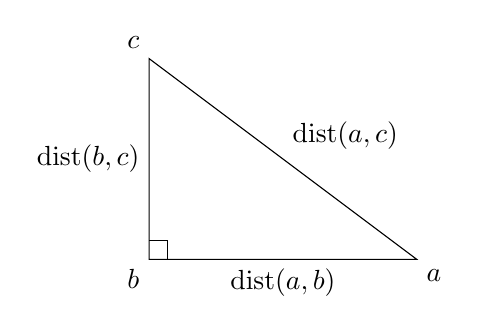
\begin{tikzpicture}[scale=0.85]
  \coordinate (b) at (0, 0);
  \coordinate (a) at (4, 0);
  \coordinate (c) at (0, 3);
  \draw (a) -- (b) -- (c) -- cycle;
  \draw (0.28, 0) -- (0.28, 0.28) -- (0, 0.28);
  \node[below left] at (b) {$b$};
  \node[below right] at (a) {$a$};
  \node[above left] at (c) {$c$};
  \node[below] at (2, 0) {$\mathrm{dist}(a, b)$};
  \node[left] at (0, 1.5) {$\mathrm{dist}(b, c)$};
  \node[above right] at (2, 1.5) {$\mathrm{dist}(a, c)$};
\end{tikzpicture}
